\documentclass[12pt,a4paper]{report}

\usepackage[utf8]{inputenc}
\usepackage[romanian]{babel}
\usepackage{graphicx}
\usepackage{amsmath}
\usepackage{amsfonts}
\usepackage{amssymb}
\usepackage{hyperref}
\usepackage{tocbibind} % Include "Bibliography" în cuprins
\usepackage{titlesec} % Pentru a centra titlurile capitolelor și secțiunilor
\usepackage{enumitem} % Liste personalizate
\usepackage{cite} 
\bibliographystyle{plainnat}
\bibliographystyle{plain}

\usepackage[numbers]{natbib}
\titleformat{\chapter}[display]
  {\normalfont\huge\bfseries\centering} % Formatare pentru titlurile capitolelor
  {\chaptername\ \thechapter}{20pt}{\Huge}

\titleformat{\section}
  {\normalfont\Large\bfseries} % Formatare pentru titlurile secțiunilor
  {\thesection}{1em}{}

\titleformat{\subsection}
  {\normalfont\large\bfseries} % Formatare pentru titlurile subsecțiunilor
  {\thesubsection}{1em}{}
\begin{document}

% Prima pagina de titlu

\begin{titlepage}
    \begin{center}
\begin{figure}[h!]
\vspace{-20pt}
\begin{center}
\includegraphics[width=100pt]{FMI-03.png}
\end{center}
\end{figure}


{\large{\bf UNIVERSITATEA DE VEST DIN TIMI\c SOARA

FACULTATEA DE MATEMATICĂ ȘI INFORMATICĂ

PROGRAM DE STUDII DE MASTERAT: Inginerie Software}}

\vspace{30pt}
{\large{\bf MEMBRII ECHIPEI: Potopea Mihaela Teodora, Stan Anamaria, Lunga Denisa, Boeriu Lavinia}}

\vspace{120pt}
{\huge {\bf Prezentare MiniSat  }}

\vspace{160pt}
\end{center}
\vfill
\begin{center}
{\bf TIMI\c SOARA

2024}
\end{center}

\end{titlepage}








% Abstractul
\chapter*{Abstract}
\addcontentsline{toc}{chapter}{Abstract} % Adaugă Rezumatul în cuprins
Acest raport prezintă o analiză aprofundată a solverului SAT MiniSat, incluzând procesul de instalare, configurare și utilizare pentru rezolvarea problemei satisfiabilității propoziționale (SAT). Obiectivul principal este de a explora performanțele MiniSat prin rularea unui benchmark selectat din competiția SAT 2024, oferind o analiză detaliată a rezultatelor experimentale obținute. În cadrul acestui proiect, au fost identificate și examinate algoritmii principali utilizați de MiniSat pentru rezolvarea problemelor SAT, incluzând algoritmul DPLL (Davis-Putnam-Logemann-Loveland) și CDCL (Conflict-Driven Clause Learning).
Prin analizarea acestor algoritmi, raportul evidențiază atât structura și funcționalitățile de bază ale MiniSat, cât și posibile îmbunătățiri care ar putea crește eficiența și scalabilitatea solverului în fața instanțelor complexe. Sunt propuse modificări ale acestor algoritmi pentru a optimiza performanțele, alături de sugestii pentru integrarea unor tehnici avansate de enumerare și învățare din conflicte. Structura internă și funcționarea solverului MiniSat sunt documentate cu ajutorul unor diagrame UML și a altor elemente de inginerie software, pentru a oferi o înțelegere clară asupra componentelor esențiale și a relațiilor dintre ele.
Raportul include, de asemenea, o secțiune dedicată provocărilor întâmpinate pe parcursul experimentelor, precum și soluțiile adoptate pentru depășirea acestora, cum ar fi dificultăți în configurarea mediului, complexitatea algoritmică și optimizarea procesului de rulare a benchmark-urilor. Codul și documentația detaliată a proiectului, incluzând raportul complet și îmbunătățirile propuse, sunt disponibile pe GitHub pentru replicare și evaluare ulterioară. Astfel, proiectul oferă atât o resursă practică pentru utilizarea MiniSat, cât și o bază teoretică solidă pentru explorarea aprofundată a algoritmilor SAT.




\tableofcontents

\chapter{Introducere}
Soluționarea problemelor de satisfiabilitate reprezintă o provocare fundamentală în domeniul informaticii teoretice, cu aplicații variate în inteligența artificială, verificarea modelului și optimizarea combinatorială. Scopul acestui raport este de a evalua performanța MiniSat, un SAT solver eficient, având implementați algoritmi avansați precum DPLL (Davis-Putnam-Logemann-Loveland) și CDCL (Conflict-Driven Clause Learning), MiniSat este un instrument vital pentru cercetarea satisfiabilității.\cite{b5}

În prima parte a acestui raport, vom prezenta problema studiată și de ce este necesară rezolvarea satisfiabilității. Ulterior vor fi discutate și analizate provocările întâmpinate la modul în care a fost instalat MiniSat și despre modul în care am efectuat teste pentru a stabili un standard. Vor fii dezbătute idei principale despre rezultate, subliniind performanța MiniSat în fața diferitelor probleme și limitări.\cite{b6}

Raportul va examina, de asemenea, algoritmii MiniSat utilizați pentru a rezolva problemele SAT. Vor fi examinate  modul în care funcționează algoritmii DPLL și CDCL, precum și modul în care aceștia pot fi îmbunătățiți pentru a crește eficiența solverului. În plus, vor fi discutate obstacolele care apar în utilizarea și adaptarea acestor algoritmi, oferind o imagine a complexității problemelor SAT și a modurilor în care acestea pot fi rezolvate.\cite{b7}

În cele din urmă, acest raport subliniază evoluția noastră cu MiniSat și ne ajută să înțelegem mai bine tehnicile avansate utilizate pentru a rezolva problemele de satisfacție. Acest lucru ne ajută să îmbunătățim instrumentele existente și să deschidem noi drumuri de cercetare în acest domeniu dinamic. Proiectul nostru, care include codul sursă și raportul complet, este accesibil pe GitHub. Acest lucru ne permite să obținem acces la resursele și rezultatele obținute.
\cite{b8}
\cite{b9}


\newpage


\section{Descrierea Problemei}
Provocarea satisfiabilității propoziționale este esențială în domeniul informaticii, având impact în diverse domenii precum inteligența artificială, optimizarea combinatorială și verificarea modelului. Această dificultate constă în a identifica dacă există o asignare a valorilor de adevăr care să îndeplinească o formulă logică exprimată în forma sa conjunctivă. Niciun algoritm cunoscut nu poate rezolva toate instanțele problemei în timp polinomial, ceea ce atrage interesul cercetătorilor pentru soluționarea eficientă a problemelor SAT. Rezolvarea problemei SAT este crucială și pentru crearea de soluționatori, precum MiniSat, care pot gestiona și rezolva cu eficiență instanțele din competițiile actuale și aplicațiile practice.

Algoritmul DPLL folosește o combinație de decizii și propagări pentru a reduce spațiul de căutare prin determinarea succesivă a valorilor literale. Prin aceste decizii, DPLL reduce dimensiunea problemei și elimină literalele care nu contribuie la soluția finală. Algoritmul este eficient pentru probleme de dimensiuni mai mici, dar când vine vorba de instanțe complexe, cum ar fi cele din competițiile SAT actuale, abordările standard nu sunt suficiente. Din această cauză, CDCL a fost introdus ca o extensie a DPLL pentru a îmbunătăți procesul de căutare și pentru a reduce spațiul de căutare prin învățarea din conflicte.

CDCL se bazează pe un proces de învățare din conflicte, care constă în identificarea și memorarea conflictelor întâlnite în timpul căutării. Când solverul detectează un conflict, acesta încearcă să identifice clauza care a dus la conflict și să o stocheze pentru a evita revizuirea aceleiași ramuri a arborelui de căutare în viitor. Această metodă este cunoscută sub numele de „învățare din conflicte” și permite solverului să reducă semnificativ numărul de decizii pe care trebuie să le ia pentru a ajunge la soluția corectă. Aceasta este o tehnică esențială pentru a face față problemelor de mare complexitate și este folosită cu succes de MiniSat și alți solvers moderni de SAT.


În proiect, analiza MiniSat a inclus realizarea de experimente pe benchmark-uri pentru a evalua performanța solver-ului în rezolvarea problemelor complexe. În timpul testelor s-a constatat că MiniSat are o structură internă bine organizată care utilizează eficient resursele disponibile pentru a maximiza eficiența de procesare. Studiile au arătat că MiniSat este eficient în rezolvarea rapidă a problemelor de dimensiuni medii și mari, făcându-l util în cercetare. De asemenea, testele au arătat că algoritmii folosiți de MiniSat pot gestiona cu succes situații extrem de complicate datorită capacității lor de a învăța din conflicte.

De asemenea, câteva provocări au fost întâmpinate. Una dintre acestea a fost legată de instalarea și setarea mediului MiniSat pentru rularea testelor de referință. De asemenea, a fost dificil să optimizăm procesul de testare, deoarece a trebuit să ajustăm setările solverului pentru a obține rezultate bune. În această situație, un alt aspect semnificativ al proiectului a fost analiza modului în care algoritmii esențiali ai MiniSat, precum DPLL și CDCL, pot fi îmbunătățiți pentru a spori eficiența și capacitatea de scalabilitate a solverului în fața provocărilor complexe.

Pentru îmbunătățirea DPLL, ar fi utilă integrarea unor tehnici de reducere a spațiului de căutare, cum ar fi euristicile avansate pentru alegerea variabilelor și a valorilor de adevăr. Euristicile de alegere a variabilelor sunt cruciale în reducerea timpului de căutare, iar tehnici precum „Variable State Independent Decaying Sum” (VSIDS) sau „Exponential Moving Average” (EMA) pot fi introduse pentru a ajuta solverul să ia decizii mai inteligente. În plus, tehnici precum eliminarea clauzelor redundante sau simplificarea formulei înainte de a începe procesul de căutare pot contribui semnificativ la îmbunătățirea performanței algoritmului DPLL.

În cazul CDCL, una dintre modalitățile de îmbunătățire constă în optimizarea procesului de învățare din conflicte. De exemplu, introducerea unor strategii de eliminare a clauzelor învățate care nu mai sunt relevante sau care sunt rareori utilizate poate ajuta la reducerea dimensiunii memoriei și la accelerarea procesului de căutare. Aceasta este o provocare, deoarece trebuie păstrate doar clauzele care contribuie în mod direct la găsirea soluțiilor, iar identificarea acestora necesită un sistem complex de evaluare a utilității fiecărei clauze învățate. În plus, introducerea unor tehnici de învățare mai sofisticate, cum ar fi analiza avansată a arborilor de conflicte sau utilizarea unor algoritmi de învățare automată pentru a anticipa conflictele viitoare, poate duce la o îmbunătățire semnificativă a performanței CDCL.

Pe lângă îmbunătățirile algoritmice, documentația proiectului MiniSat include și diagrame UML și alte instrumente de inginerie software pentru a oferi o înțelegere clară asupra structurii interne a solverului și a relațiilor dintre componentele sale. Aceste diagrame au ajutat la elucidarea modului în care funcționează MiniSat și la identificarea punctelor cheie de optimizare. De exemplu, analiza diagramelor de clasă a evidențiat interacțiunile dintre diferitele module ale solverului, iar diagramele de secvență au arătat fluxul operațiunilor de căutare și învățare din conflicte.

\newpage

\chapter{Pașii Instalării MiniSat}
Pentru instalarea MiniSat pe laptopurile personale, am folosit Windows Subsystem for Linux (WSL). 

1.Primul pas in instalarea MiniSat-ului este activarea WSL:
\vspace{5pt}

 \begin{itemize}
 \item \textbf{Se deschide PowerShell ca administrator.} 

 \item \textbf{Se introduce următoarea comanda, care instalează automat cea mai recenta versiune a WSL și va descarca și Ubuntu:} 
 \vspace{5pt}
 \begin{itemize}
     \item \textbf{wsl --install}
 \end{itemize}

\item \textbf{După ce instalarea este completa, trebuie repornit laptopul.} 

\end{itemize}
 



2.Al doilea pas este configurarea WSL și Ubuntu:
 \begin{itemize}
 \item \textbf{Deschidem Ubuntu din meniul de start și se vor urma instrucțiunile necesare pentru setarea unui utilizator și a parolei.} 

\end{itemize}

3. Ultimul pas pentru instalare:

\begin{itemize}
 \item \textbf{Se va deschide terminalul WSL și se vor rula următoarele comenzi:}
\begin{itemize}
 \item {sudo apt-get update}
\item {sudo apt-get install minisat}

\end{itemize}
\end{itemize}

4.După instalare, verifică dacă MiniSat funcționează introducând comanda:
\begin{itemize}
\begin{itemize}
 \item {minisat}
\end{itemize}
\end{itemize}



\section{Problemele întâmpinate la instalarea MiniSat}
Până la obținerea rezultatului final, care a constat în instalarea cu succes a MiniSat, am întâmpinat diverse probleme. Acestea au fost soluționate printr-o documentare temeinică realizată pe internet.
 \begin{itemize}
 \item \textbf{P1: Lipsa utilitarelor de dezvoltare necesare pentru compilare } 
 Instalarea MiniSat este destul de dificilă dacă nu sunt utilizate utilitare de dezvoltare precum make sau un compilator C++ adecvat, cum ar fi g++ sau clang. Rularea fișierului Makefile, care automatizează procesul de compilare, necesită utilizarea acestor programe. Lipsa acestora poate provoca erori, cum ar fi make: comanda nu găsită, care indică faptul că sistemul de operare nu este pregătit pentru compilare. Sistemele mai simple sau mașinile virtuale care nu au utilitarele dezvoltatorilor preinstalate întâmpină frecvent această problemă. Soluția implică utilizarea anumitor comenzi pentru sistemul de operare pentru instalarea instrumentelor de dezvoltare, cum ar fi sudo apt install build-essential pentru distribuțiile Debian sau xcode-select --install pentru macOS. Prin urmare, se asigură că toate dependențele care sunt necesare pentru compilarea MiniSat sunt disponibile.

 \item \textbf{P2: Incompatibilități sau fișiere lipsă în sursa MiniSat} 
Uneori există incompatibilități între versiunea compilatorului utilizat și codul sursă MiniSat, ceea ce provoacă erori în timpul compilării, care sunt o altă problemă majoră. Aceste erori pot include mesaje precum fatal error: no such file or directory sau probleme legate de standardele actuale ale limbajului C++, cum ar fi utilizarea improprie a funcționalităților introduse în C++11. Utilizatorii pot descărca uneori o sursă MiniSat incompletă sau învechită. Pentru a rezolva aceste probleme, se recomanda să se descarce codul din repository-ul oficial GitHub, care oferă versiunea actualizată. De asemenea, este posibila verificarea compatibilitatii compilatorului folosind comanda g++ -version. În plus, actualizarea compilatorului garantează suportul pentru toate caracteristicile moderne necesare compilării fără erori.


\item \textbf{P3: Configurarea incorectă a binarelor MiniSat} 
Atunci când procesul de compilare este finalizat, o problemă frecventă este incapacitatea de a executa MiniSat direct din terminal. Acest lucru se datorează unei configurări inadecvate a variabilei de mediu PATH. În aceste situații, chiar dacă executabilul a fost creat cu succes, comanda minisat poate returna eroarea comanda nu găsită. Această problemă rezultă din faptul că calea de căutare a sistemului de operare nu include directorul unde se află binarul MiniSat. Soluția include mutarea binarului într-un director global accesibil, cum ar fi /usr/local/bin, sau adăugarea directorului de compilare manual în variabila PATH. Este posibil să se configureze permanent această variabilă prin modificarea fișierelor.bashrc sau.zshrc, ceea ce facilitează utilizarea în orice sesiune.

\end{itemize}


\chapter{Rezultate Rulare Benchmark}

Pentru a evalua performanța solverului Minisat, am utilizat un set de benchmark-uri în format CNF, provenind din competiția SAT 2024. Scopul rularii benchmarkurilor a fost sa analizeze timpul de execuție, utilizarea memoriei și capacitatea solverului de a determina corect dacă o problema este satisfiabila (SAT) sau nesatisfiabila (UNSAT). Benchmarkurile selectate fac parte din familia Hamiltonian și variază în dimensiune.
\newline
\newline
Pentru a rula benchmark-urile, folosim următorul link pentru a le descărca: 
\href{https://benchmark-database.de/?track=main_2024}{https://benchmark-database.de/?track=main\_2024}. 
Aici sunt afișate multiple familii și teste pentru rulare. În funcție de familia pe care dorim să o rulăm, putem să căutăm în bara de căutare denumirea fiecărei familii. În cazul familiei \textit{Hamiltonian}, vom căuta: \texttt{track=main\_2024 and family like hamiltonian}, 
pentru a ne afișa doar fișierele familiei din competiția SAT 2024. 
În continuare, se descarcă fiecare fișier în parte, în total 40 de fișiere.
Solverul \textit{MiniSat} se va rula utilizând următoarea comandă:
\begin{verbatim}minisat input.cnf output.out > output.stats
\end{verbatim}
În fișierul de intrare \texttt{input.cnf} găsim descrierea problemei SAT, în timp ce fișierele de ieșire \texttt{output.out} și \texttt{output.stats} includ rezultatul (\texttt{SAT/UNSAT}) și statistici de performanță, cum ar fi timpul de execuție, numărul de restarturi și memoria utilizată.
\newline
\newline
Rezultatele benchmark-urilor au arătat că \textit{MiniSat} rezolvă eficient problemele de dimensiuni mici și medii. Problemele \texttt{UNSAT} au fost, în general, mai dificil de rezolvat, necesitând mai multe restarturi și având un număr mai mare de conflicte. În medie, solverul a utilizat între 15 și 47 MB de memorie și demonstrează eficiență în utilizarea resurselor.
\newline
Pe baza acestor rezultate, \textit{MiniSat} s-a dovedit a fi potrivit pentru aplicații care necesită soluționarea rapidă a problemelor de dimensiuni rezonabile, dar poate necesita optimizări sau utilizarea unor algoritmi mai avansați pentru probleme industriale.


\begin{tabular}{ |p{1cm}||p{4cm}|p{3cm}|p{3cm}|p{3cm}|  }
 \hline
 \multicolumn{4}{|c|}{Familia Hemiltonian} \\
 \hline
 Nr crt.& Nume Benchmark & Timp (s)& SAT/UNSAT & Memory used(MB)\\
 \hline

1 & x9-08014.sat.sanitized &2.160& UNSAT & 17\\\  
2 & x9-08075.sat.sanitized &2.160& UNSAT & 15\\\  
3 & x9-09004.sat.sanitized &2.160& UNSAT & 25\\\  
4 & x9-09007.sat.sanitized &2.160& UNSAT & 21\\\  
5 & x9-09014.sat.sanitized &2.160& UNSAT & 22\\\  
6 & x9-09024.sat.sanitized &2.160& UNSAT & 18\\\  
7 & x9-09047.sat.sanitized &2.160& UNSAT & 19\\\  
8 & x9-09051.sat.sanitized &2.160& UNSAT & 28\\\  
9 & x9-09054.sat.sanitized &2.160& SAT & 19\\\  
10 & x9-09057.sat.sanitized &2.160& UNSAT & 23\\\  
11 & x9-09076.sat.sanitized &2.160& UNSAT & 25\\\  
12 & x9-09098.sat.sanitized &2.160& UNSAT & 23\\\  
13 & x9-10002.sat.sanitized &2.160& UNSAT & 46\\\  
14 & x9-10007.sat.sanitized &2.160& UNSAT & 39\\\  
15 & x9-10014.sat.sanitized &2.160& SAT & 25\\\  
16 & x9-10027.sat.sanitized &2.160& SAT & 29\\\  
17 & x9-10031.sat.sanitized &2.160& UNSAT & 48\\\  
18 & x9-10038.sat.sanitized &2.160& SAT & 24\\\  
19 & x9-10051.sat.sanitized &2.160& UNSAT & 44\\\  
20 & x9-10076.sat.sanitized &2.160& UNSAT & 35\\\  
21 & x9-10083.sat.sanitized &2.160& UNSAT & 35\\\  
22 & x9-10084.sat.sanitized &2.160& UNSAT & 41\\\  
23 & x9-10093.sat.sanitized &2.160& UNSAT & 40\\\  
24 & x9-10096.sat.sanitized &2.160& UNSAT & 36\\\  
25 & x9-10098.sat.sanitized &2.160& SAT & 18\\\  
26 & x9-11034.sat.sanitized &2.160& SAT & 43\\\  
27 & x9-11053.sat.sanitized &2.160& SAT & 26\\\  
28 & x9-11062.sat.sanitized &2.160& SAT & 39\\\  
29 & x9-11077.sat.sanitized &2.160& SAT & 34\\\  
30 & x9-11088.sat.sanitized &2.160& SAT & 33\\\  
31 & x9-11093.sat.sanitized &2.160& SAT & 20\\\  
32 & x9-11094.sat.sanitized &2.160& SAT & 23\\\  
33 & x9-12001.sat.sanitized &2.160& SAT & 42\\\  
34 & x9-12014.sat.sanitized &2.160& SAT & 25\\\  
35 & x9-12021.sat.sanitized &2.160& SAT & 38\\\  
36 & x9-12035.sat.sanitized &2.160& SAT & 43\\\  
37 & x9-12063.sat.sanitized &2.160& SAT & 39\\\  
38 & x9-12087.sat.sanitized &2.160& SAT & 25\\\  
39 & x9-12092.sat.sanitized &2.160& SAT & 31\\\  
40 & x9-12098.sat.sanitized &2.160& SAT & 47\\\
\hline
 
\end{tabular}


\chapter{Fluxul MiniSat}
\section{Use Case Diagram}
Cu ajutorul acestei diagrame se identifică caracteristicile principale ale MiniSat, cum ar fi rezolvarea problemelor SAT, analizarea fișierelor de intrare și soluționarea conflictelor. Aceasta utilizează modele de interacțiune utilizator/sistem și descrie modul în care părțile externe, cum ar fi cadrele universitare, dezvoltatorii sau aplicațiile, se implică în funcțiile esențiale ale MiniSat. Se clarifică limitele sistemului, atrăgând atenția asupra sarcinilor pe care MiniSat le gestionează și asupra celor care sunt gestionate de alte persoane sau sisteme.

\begin{figure}[h]
    \centering
    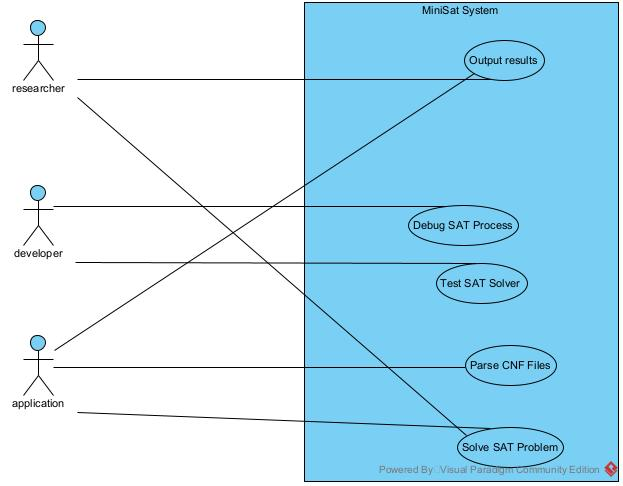
\includegraphics[width=0.5\linewidth]{minisat_1.jpg}
    \caption{Use case diagram}
    \label{fig:enter-label}
\end{figure}
\\
\section{Class Diagram}
Obiectivele principale intr-o diagramă de clase sunt structura fundamentală a MiniSat-ului, inclusiv componentele sale principale, cum ar fi Literal, Clause, Database, Propagator și interacțiunile lor, care sunt reprezentate de arhitectura de bază, care evidențiază, de asemenea, datele și operațiunile importante și direcționează implementarea orientată spre obiect.Evidențiază informațiile și activitățile importante: afișează proprietățile și metodele fiecărei clase și ajută dezvoltatorii să înțeleagă structura componentelor MiniSat, acționând ca un plan pentru construirea software-ului.

\begin{figure}[h]
    \centering
    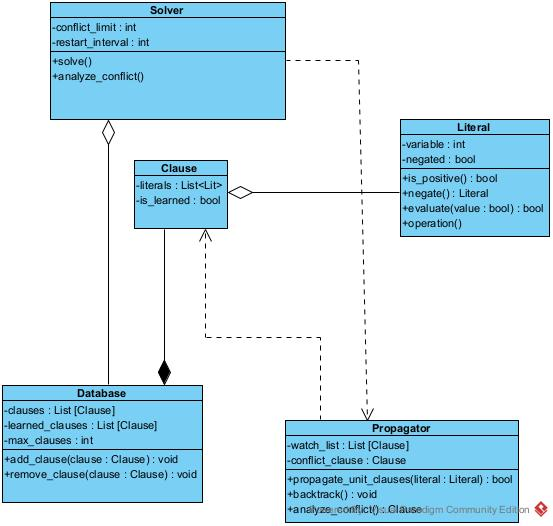
\includegraphics[width=0.5\linewidth]{minisat_2.jpg}
    \caption{Class diagram}
    \label{fig:enter-label}
\end{figure}

\section{Sequence Diagram}
Obiectivele principale ale diagramei de secvențe sunt detalierea fluxului de execuție, prezentarea interacțiunilor dintre componente și, bineînțeles, evidențierea comportamentului dinamic.Ilustrează modul în care MiniSat procesează pas cu pas o cerere de rezolvare SAT, de la analizarea datelor de intrare până la emiterea rezultatelor.Explică modul în care componente precum Solver, Database și Propagator fac schimb de mesaje pentru a îndeplini sarcini specifice.De asemenea, descrie ordinea operațiunilor pentru scenarii cheie, cum ar fi rezolvarea conflictelor sau backtracking.

\begin{figure}[h]
    \centering
    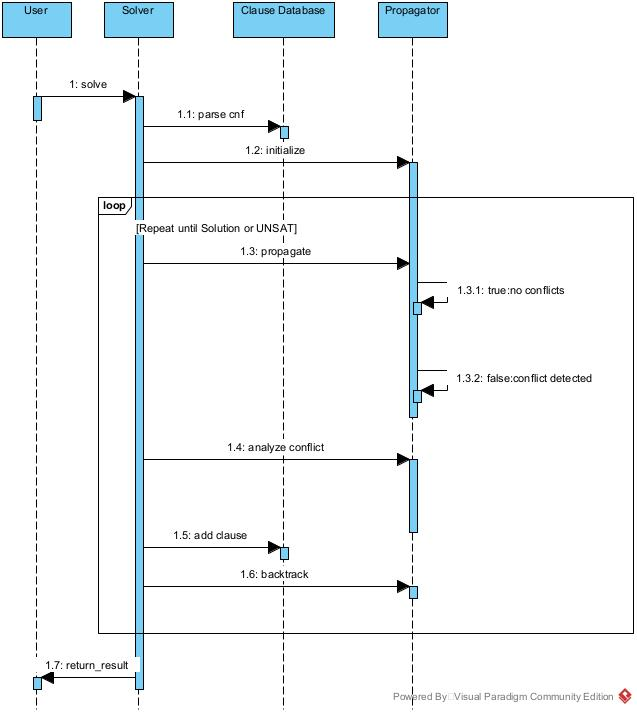
\includegraphics[width=0.5\linewidth]{minisat_3.jpg}
    \caption{Sequence diagram}
    \label{fig:enter-label}
\end{figure}

\section{Activity Diagram}
Diagrama de activitate prezintă ca biective principale modelarea fluxului de soluționare SAT, identificarea punctelor de decizie și evidențierea punctelor de decizie.Descrie fluxul logic al operațiunilor MiniSat, inclusiv propagarea, detectarea conflictelor și backtracking.Clarifică punctele critice de ramificare, cum ar fi dacă este detectat un conflict sau dacă toate variabilele au fost atribuite.Arată sarcini simultane, cum ar fi verificarea mai multor clauze în timpul propagării.
\begin{figure}[h]
    \centering
    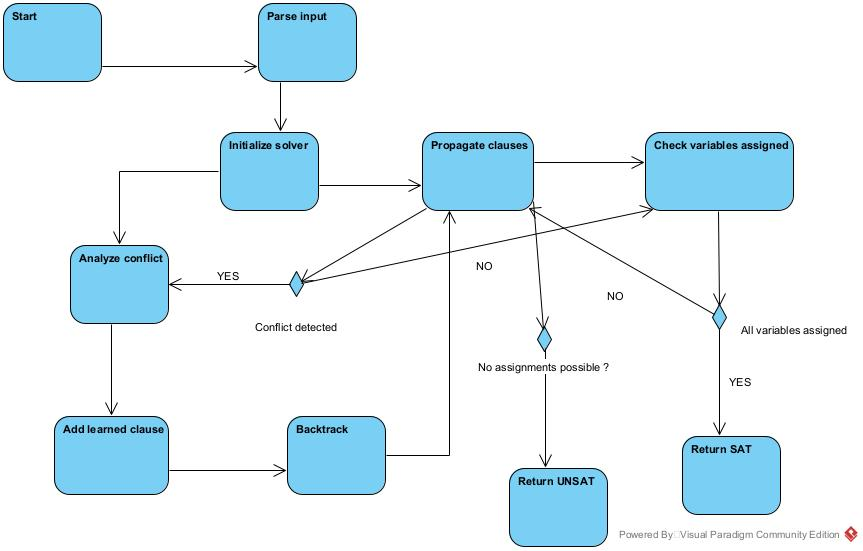
\includegraphics[width=0.5\linewidth]{minisat_4.jpg}
    \caption{Activity diagram}
    \label{fig:enter-label}
\end{figure}

 \cite{b5}


\chapter{Documentarea codului}

\section*{CDCL (Conflict-Driven Clause Learning)}
CDCL este algoritmul central folosit în \textit{MiniSat} pentru rezolvarea problemei SAT. Este o extensie a DPLL, îmbunătățită prin mecanisme precum învățarea de clauze și decizii euristice.

\subsection*{Părți esențiale implementate în \textit{MiniSat}}
\begin{itemize}
    \item \textbf{Solver.cc și Solver.h:}
    \begin{itemize}
        \item \textit{Propagarea unitară (Unit Propagation)}: Propagarea este implementată aici și joacă un rol esențial în CDCL. Se face traversarea clauzelor pentru a găsi literaluri care trebuie să fie adevărate din cauza altor alegeri anterioare. Aceasta se face printr-un mecanism eficient de \textit{watched literals}. Codul corespunzător propagării este probabil în metoda \texttt{propagate()} din \texttt{Solver.cc}.
        \item \textit{Decizii euristice}: Alegerea următoarei variabile pentru evaluare este tratată aici, folosind scoruri precum \textit{VSIDS} (Variable State Independent Decaying Sum).
        \item \textit{Backjumping}: Analiza conflictelor și revenirea la punctul relevant pentru rezolvarea conflictului. Implementată în funcția \texttt{analyze()}.
        \item \textit{Învățarea de clauze}: După un conflict, \textit{MiniSat} învață o clauză pentru a preveni repetarea aceleași greșeli, prin funcția \texttt{analyze()}.
    \end{itemize}
    \item \textbf{Heap.h (din folderul \texttt{mtl}):} Folosit pentru prioritizarea variabilelor bazat pe scoruri euristice.
    \item \textbf{Vec.h (din folderul \texttt{mtl}):} Gestionarea eficientă a clauzelor și literalurilor.
    \item \textbf{SolverTypes.h:} Definește structuri de date precum \texttt{Clause}, \texttt{Literal} etc.
\end{itemize}

\section*{DPLL (Davis-Putnam-Logemann-Loveland)}
DPLL este algoritmul pe care CDCL îl extinde. Este mai simplu, fără optimizări precum învățarea de clauze și decizii bazate pe grafuri de conflict.

\subsection*{Părți esențiale implementate în \textit{MiniSat}}
\begin{itemize}
    \item \textbf{Decizii și backtracking:} DPLL folosește backtracking simplu, fără analiza conflictelor. Codul se găsește în \texttt{Solver.cc}.
    \item \textbf{Propagarea unitară:} Comună între DPLL și CDCL, implementată în funcția \texttt{propagate()} din \texttt{Solver.cc}.
    \item \textbf{Algoritmul principal DPLL:} Implementat în funcțiile de căutare recursivă din \texttt{Solver.cc}.
\end{itemize}

\section*{Analiză detaliată a metodelor}
\subsection*{Funcții cheie}

\begin{enumerate}[label=\arabic*.]
    \item \textbf{Propagarea unitară (\texttt{propagate})}  
    \textit{Locație: Solver.cc}  
    Găsește clauze unitare și actualizează starea solverului. Utilizează \textit{watched literals} pentru eficiență. Dacă rezultă o clauză goală, indică un conflict.

    \item \textbf{Analiza conflictelor (\texttt{analyze})}  
    \textit{Locație: Solver.cc}  
    În cazul unui conflict, determină cauza utilizând graful de implicații. Creează o clauză nouă (\textit{cut clause}) folosind \textit{First UIP}.

    \item \textbf{Backtracking (\texttt{backtrack}) și Backjumping}  
    \textit{Locație: Solver.cc}  
    CDCL utilizează \textit{backjumping}, revenind la nivelul relevant pentru rezolvarea conflictului.

    \item \textbf{Selecția variabilelor (\texttt{pickBranchLit})}  
    \textit{Locație: Solver.cc, Heap.h}  
    Folosește euristica \textit{VSIDS} pentru selectarea variabilelor.

    \item \textbf{Învățarea de clauze (\texttt{learnClause})}  
    \textit{Locație: Solver.cc}  
    Previne repetarea conflictelor prin adăugarea clauzelor învățate.

    \item \textbf{Simplificarea formulei (\texttt{simplify})}  
    \textit{Locație: SimpSolver.cc}  
    Aplică tehnici precum eliminarea literalurilor pure sau subsumpția clauzelor.

    \item \textbf{Funcția principală de căutare (\texttt{solve})}  
    \textit{Locație: Solver.cc}  
    Integrează propagarea, analiza conflictelor, backjumping-ul și verificarea satisfiabilității.
\end{enumerate}



\chapter{Raport de activitate în cadrul proiectului pentru fiecare membru al echipei}
Proiectul realizat se poate accesa prin link-ul: \href{https://github.com/lungadenisa/MiniSat---VF-Project}{https://github.com/lungadenisa/MiniSat---VF-Project}.De asemenea, documentarea codului se poate accesa prin link-ul:
\url{https://docs.google.com/document/d/17dpwrUJ_5nGMMfIYFlbtwOZ6_ki_n_oHQJSLbJMvhV8/edit?tab=t.0#heading=h.rgn6slwpli8g}
\section{Potopea Mihaela Teodora}
\paragraph{EMAIL:} mihaela.potopea03@e-uvt.ro

\paragraph{ATRIBUȚII:} Probleme întâmpinate la rulare și alte probleme, Latex Report

\section{Stan Anamaria}
\paragraph{EMAIL:} anamaria.stan02@e-uvt.ro

\paragraph{ATRIBUȚII:} Introducere, Descrierea problemei, Diagrame UML, Latex Report

\section{Lunga Denisa}
\paragraph{EMAIL:} denisa.lunga00@e-uvt.ro

\paragraph{ATRIBUȚII:} Instalare Minisat, Rulare benchmark, Încărcare cod pe GitHub

\section{Boeriu Lavinia}

\paragraph{EMAIL:} lavinia.boeriu02@e-uvt.ro

\paragraph{ATRIBUȚII:} Abstract, Documentare cod, Explicații prin comentarii în cod

\newpage
 











\bibliography{thesis}

\end{document}
